% !TeX spellcheck = en_GB
\documentclass[abstract,toc,los,english,11pt,glossaries]{jluthesis}

\usepackage{siunitx}

\newacronym{eas}{EAS}{Extensive Air Showers}
\newacronym{uhecr}{UHECR}{Ultra High Energy Cosmic Radiation}
\newacronym{sipm}{SiPM}{Silicon Photomultiplier}
\newacronym{adc}{ADC}{Analog Digital Converter}
\newacronym{enu}{ENU}{East, North Up}
\newacronym{com}{COM}{center of mass}
\newacronym{csda}{CSDA}{continuous-slowing-down approximation}
\newacronym{gzkl}{GZK-Limit}{Greisen–Zatsepin–Kuzmin limit}
\newglossaryentry{hadron} {name=hadron, description={subatomic particle affected by the strong interaction}}
\newglossaryentry{nucleus} {name=nucleus, plural=nuclei, description={Center of an atom}}
\bibliography{data/thesis.bib}

\topic{Real-time data analysis of distributed muon detector network}
\title[Bachelor Thesis]{Bachelor Thesis}
\author[Daniel Treffenstädt]{Daniel J.S. Treffenstädt}
\matnr{6067797}
\supervisor{Prof. Dr. Kai-Thomas Brinkmann\\Dr. Hans-Georg Zaunick}



\begin{document}
\makebeginning{
	This thesis attempts to create a real-time analysis of coincidences from timestamped detection events through a network of scintillator detectors. The goal thereby is to create an efficient way to calculate coincidences between all detector stations and hopefully identify cosmic air shower events. Ultimately this could lead to the reconstruction of primary cosmic particles which caused the events.
}

\section{Introduction}
\subsection{Cosmic Radiation}
\acrfull{uhecr} is cosmic radiation in the energy regime of $10^{18}$\,eV to $10^{20}$\,eV. Cosmic radiation has been discovered in 1912 by Viktor Hess by performing measurements with three electrometers in a balloon flight. He discovered the secondary radiation in the atmosphere which is produced through the interaction of primary cosmic radiation with the atmosphere. The cosmic radiation thereby is produced by many different sources, one of which is our sun, which produces radiation up to a few hundreds of MeV of energy. Other sources are mainly other stars, supernovae and also black holes. \\
\begin{figure}[ht!]
	\centering
	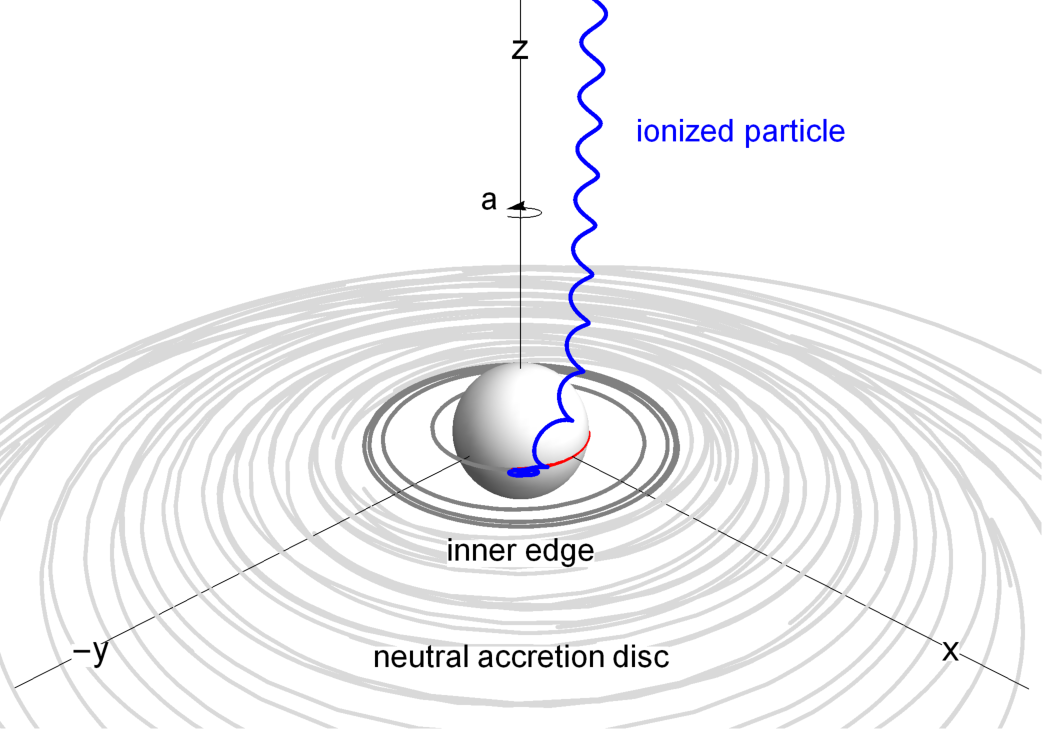
\includegraphics[width=0.5\linewidth]{data/uhecr-sm-bh}
	\caption{Trajectory of neutral particle around supermassive black hole \cite{Tursunov_2020}}
	\label{fig:uhecr-sm-bh}
\end{figure}\\
For \acrshort{uhecr}, the exact production mechanism is unknown and an area of active research, though some sources have been speculated. One such proposed mechanism is a spinning supermassive hole with a neutral particle in its accretion disk. The Orbit of this particle decays until it is close enough to the black hole so that the effective electric charge dominates and ionises the particle which causes a large acceleration\cite{Tursunov_2020}. The trajectory of the particle is shown in figure \ref{fig:uhecr-sm-bh}.\\
\begin{figure}[ht!]
	\centering
	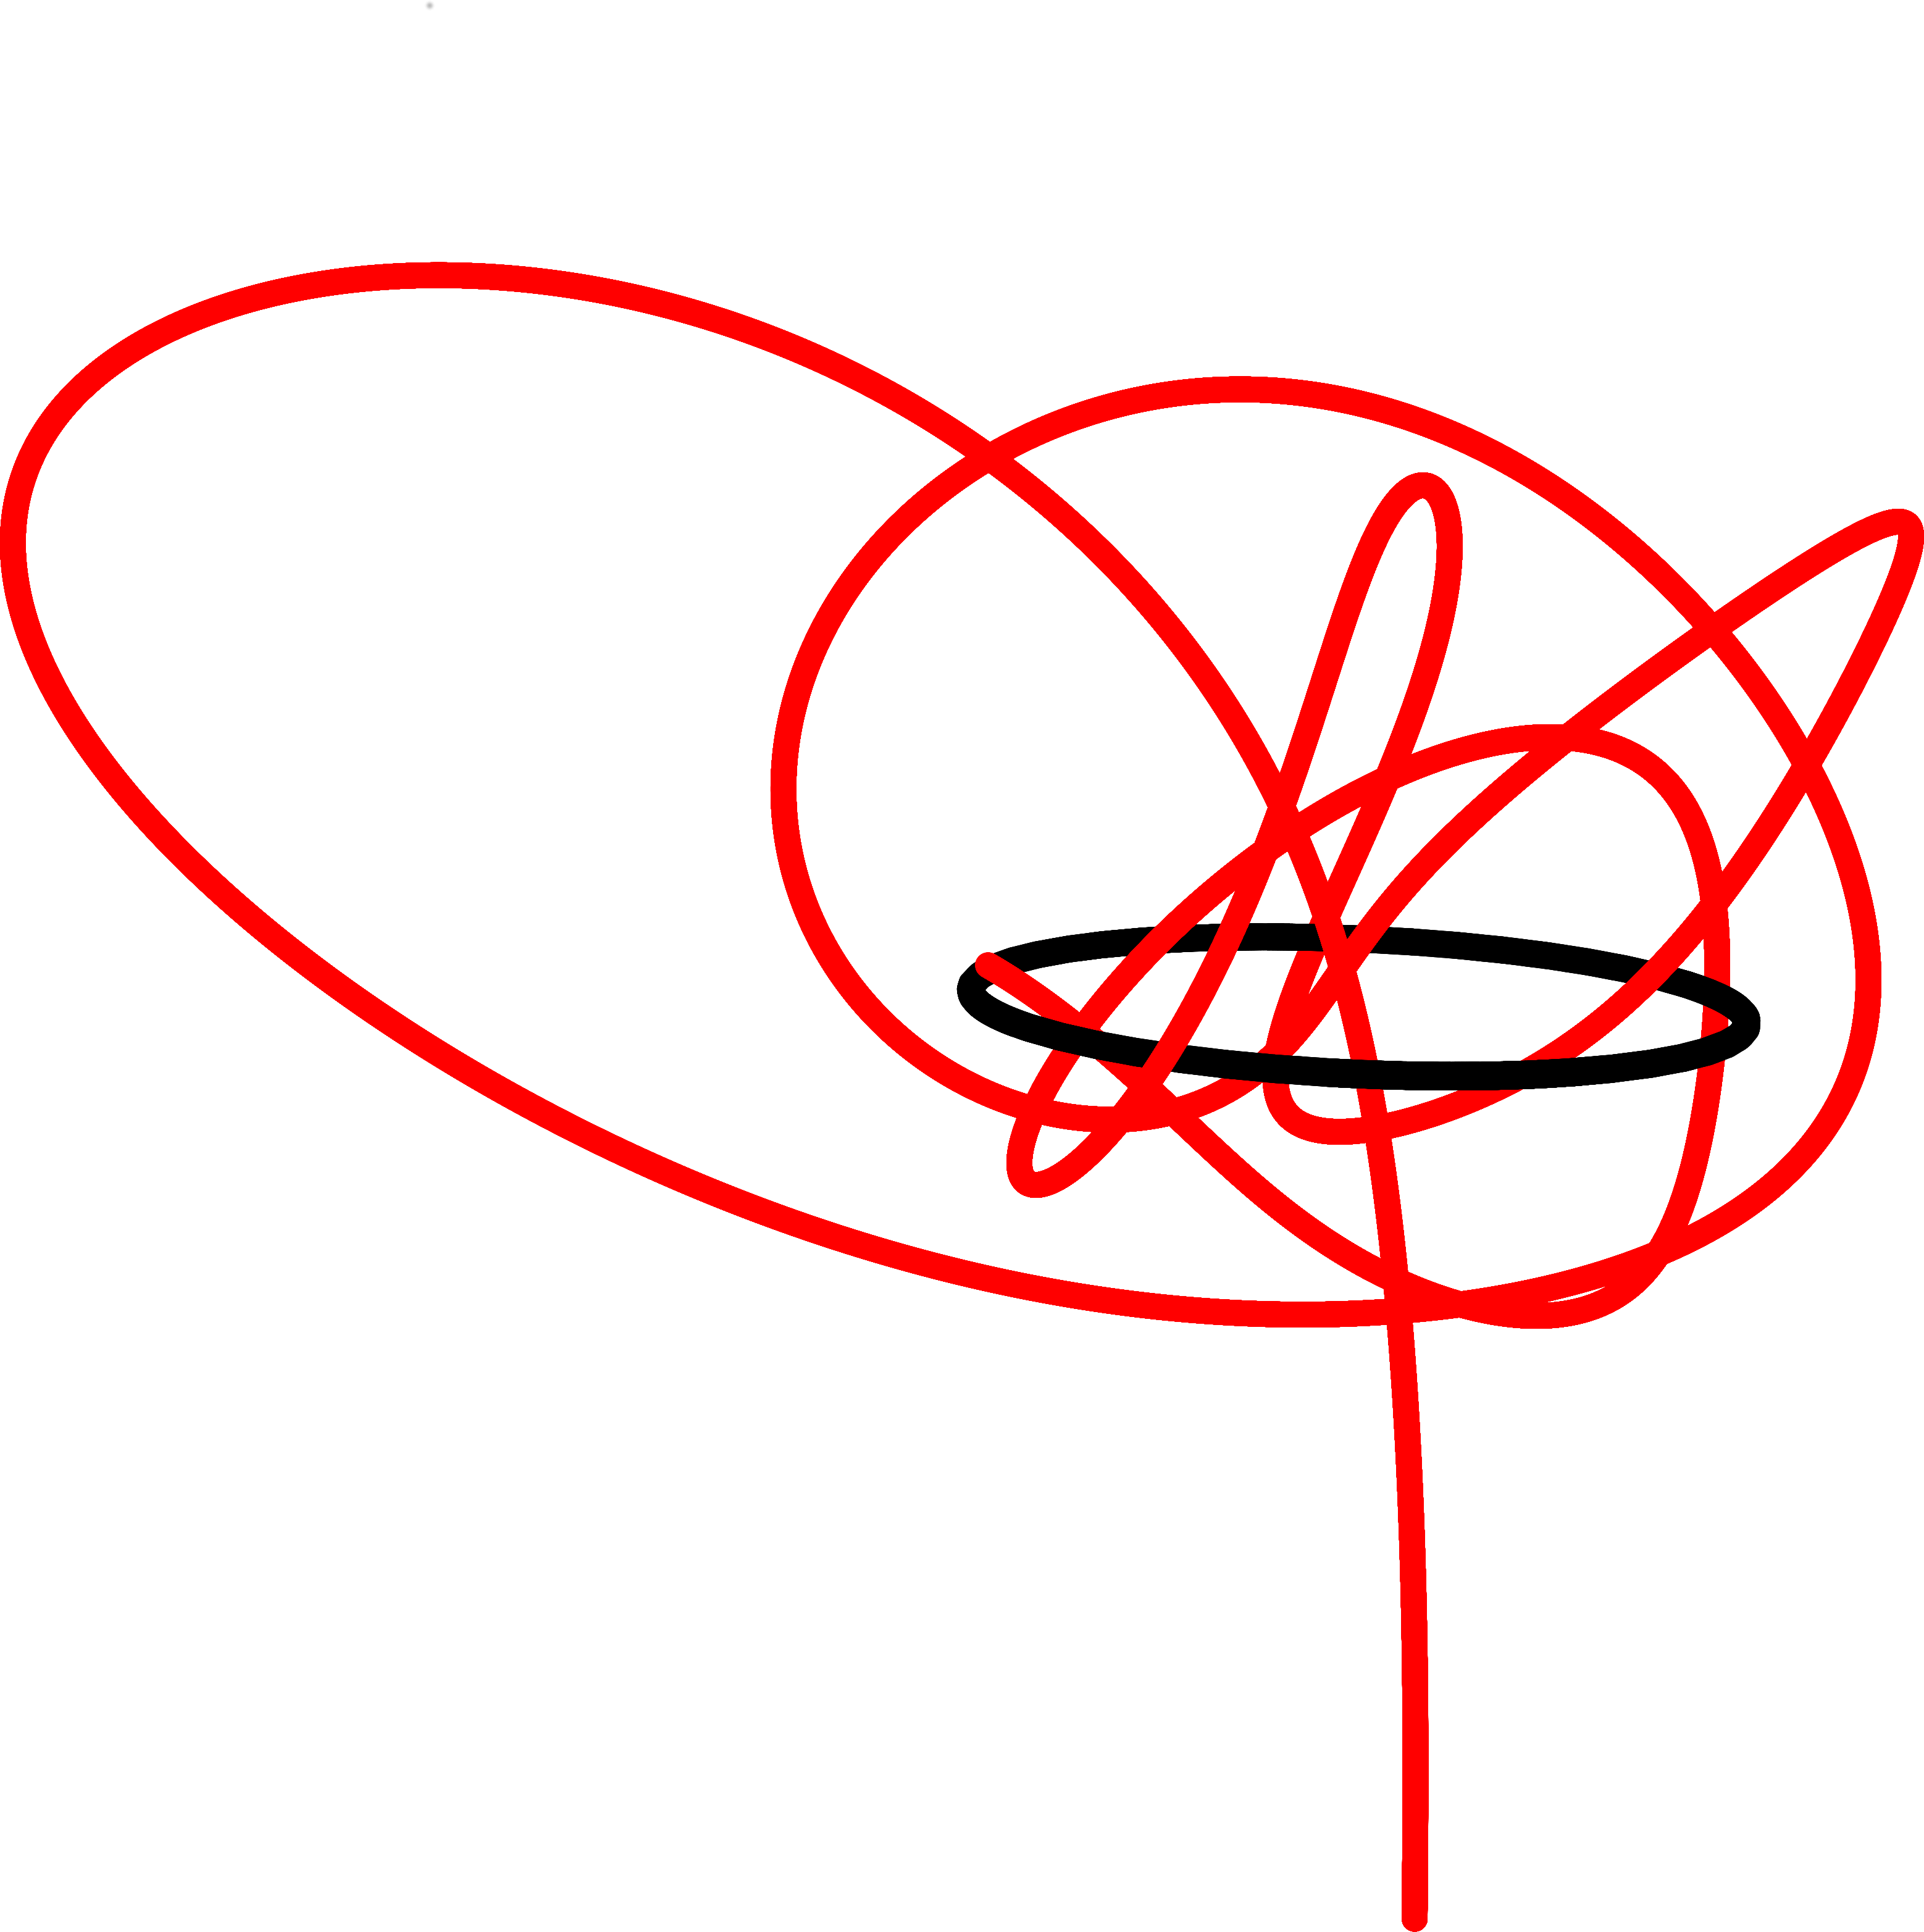
\includegraphics[width=0.4\linewidth]{data/trajectory-binary-bh}
	\caption{Possible trajectory of UHECR in Binary Black hole system \cite{Zhang2020}}
	\label{fig:trajectory-binary-bh}
\end{figure} \\
Another proposed mechanism also involves black holes, though here the particle is not produced, rather it is accelerated. This proposition requires a pair of binary black holes which are so close to each other that they move at relativistic speeds. In such a scenario a particle can experience a series of gravitational slingshots\cite{Zhang2020} around the binary black hole and finally be accelerated so much it reaches the necessary energy region to be classified as a \acrshort{uhecr}. One such series of slingshots is shown in figure \ref{fig:trajectory-binary-bh}. \\
\begin{figure}[ht!]
	\centering
	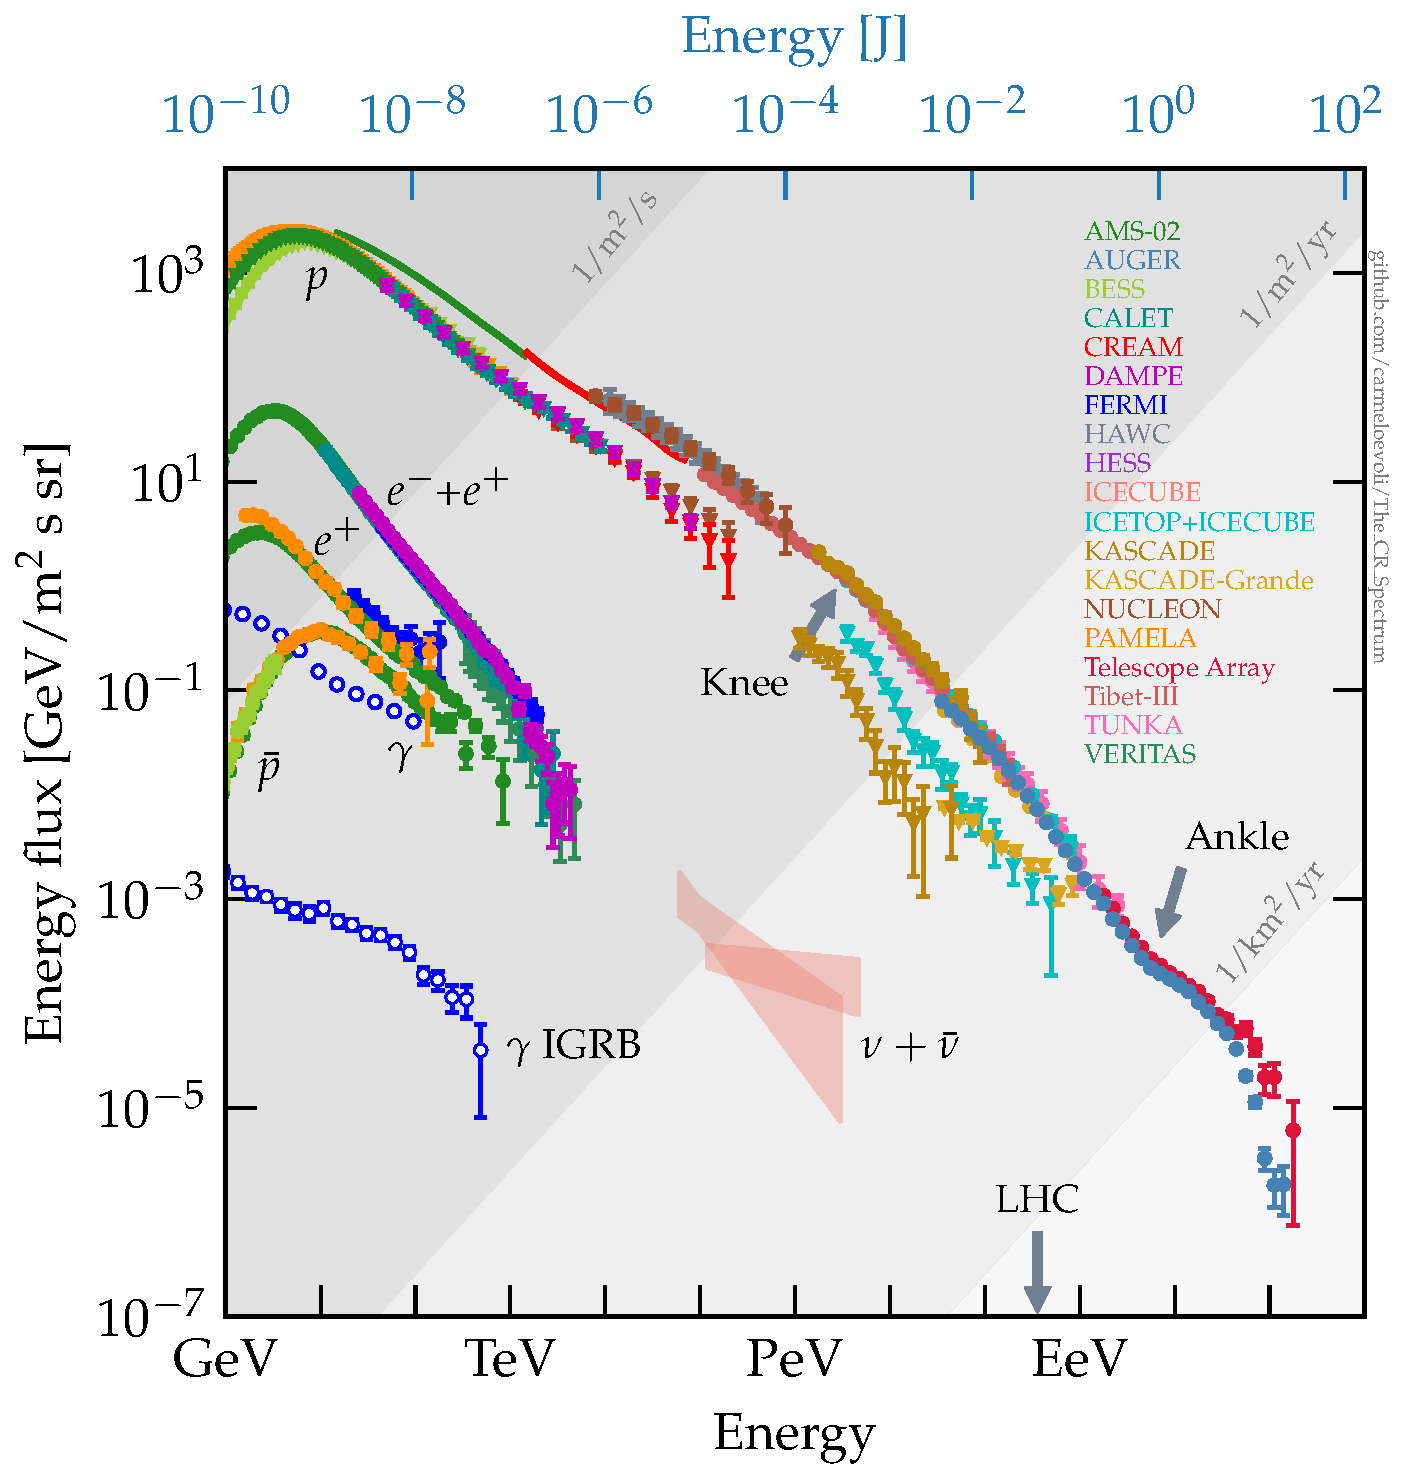
\includegraphics[width=0.5\linewidth]{data/cr_spectrum}
	\caption{Spectrum of cosmic radiation \cite{evoli_carmelo_2020_4396125}}
	\label{fig:cr_spectrum}
\end{figure} \\
The spectrum of this cosmic radiation is shown in figure \ref{fig:cr_spectrum}. There, measurements from different experiments are shown. The y axis shows the energy flux of cosmic rays in units of energy per second per square meter per solid angle $\frac{\text{GeV}}{\text{m}^2\cdot\text{s}\cdot\text{sr}}$. The x axis shows the primary energy of the cosmic rays. Notable here is the much higher number of protons as compared to all other particles by two orders of magnitude. This allows one to make the reasonable assumption that most cosmic rays are protons. \\
Notable is also that there are protons above $5\cdot10^{19}$\,eV of energy.
This is usually considered the \acrfull{gzkl}\cite{2021APh...12602526B}, a limit which arises through the interaction of protons with the microwave background radiation. This limit got its name due to its first computation by three physicists independently of each other in 1966. The violation of this limit could be explained with a proposition by the Pierre Auger Observatory that most \acrshort{uhecr} are in fact heavier nuclei than single protons \cite{thepierreaugercollaboration2017inferences}.

\subsection{Cosmic Air Showers}
In the case that a \acrshort{uhecr} interacts with air molecules in the atmosphere, a cascade of secondary particles is created. This shower can be grouped in three components. They are shown in figure \ref{fig:shower-components} and are:
\begin{itemize}
	\item Electromagnetic, photons $\gamma$ and electrons or positrons $e^\pm$
	\item Mesonic, mostly muons $\mu^\pm$
	\item Hadronic, protons $p,\bar{p}$ and neutrons $n,\bar{n}$
\end{itemize}
\begin{figure}[ht!]
	\centering
	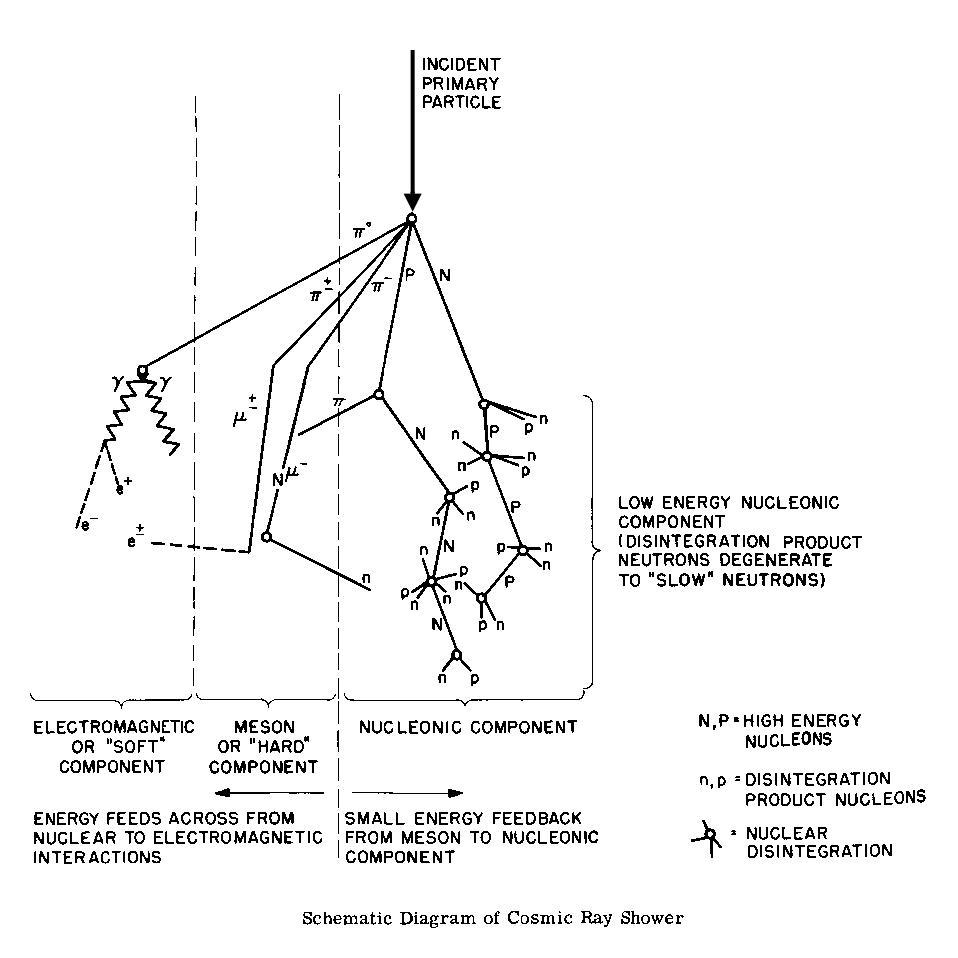
\includegraphics[width=0.6\linewidth]{data/shower-components}
	\caption{\todo{better figure!} Components of a cosmic air shower \cite{desy-zeuthen}}
	\label{fig:shower-components}
\end{figure}
A class of cosmic air showers are the \acrfull{eas}, those are showers produced by \acrshort{uhecr}. A picture of a simulated air shower produced by a primary proton is shown in figure \ref{fig:proton-shower}. This image is produced at the KIT with the simulation toolkit CORSIKA. 
\begin{figure}[ht!]
	\centering
	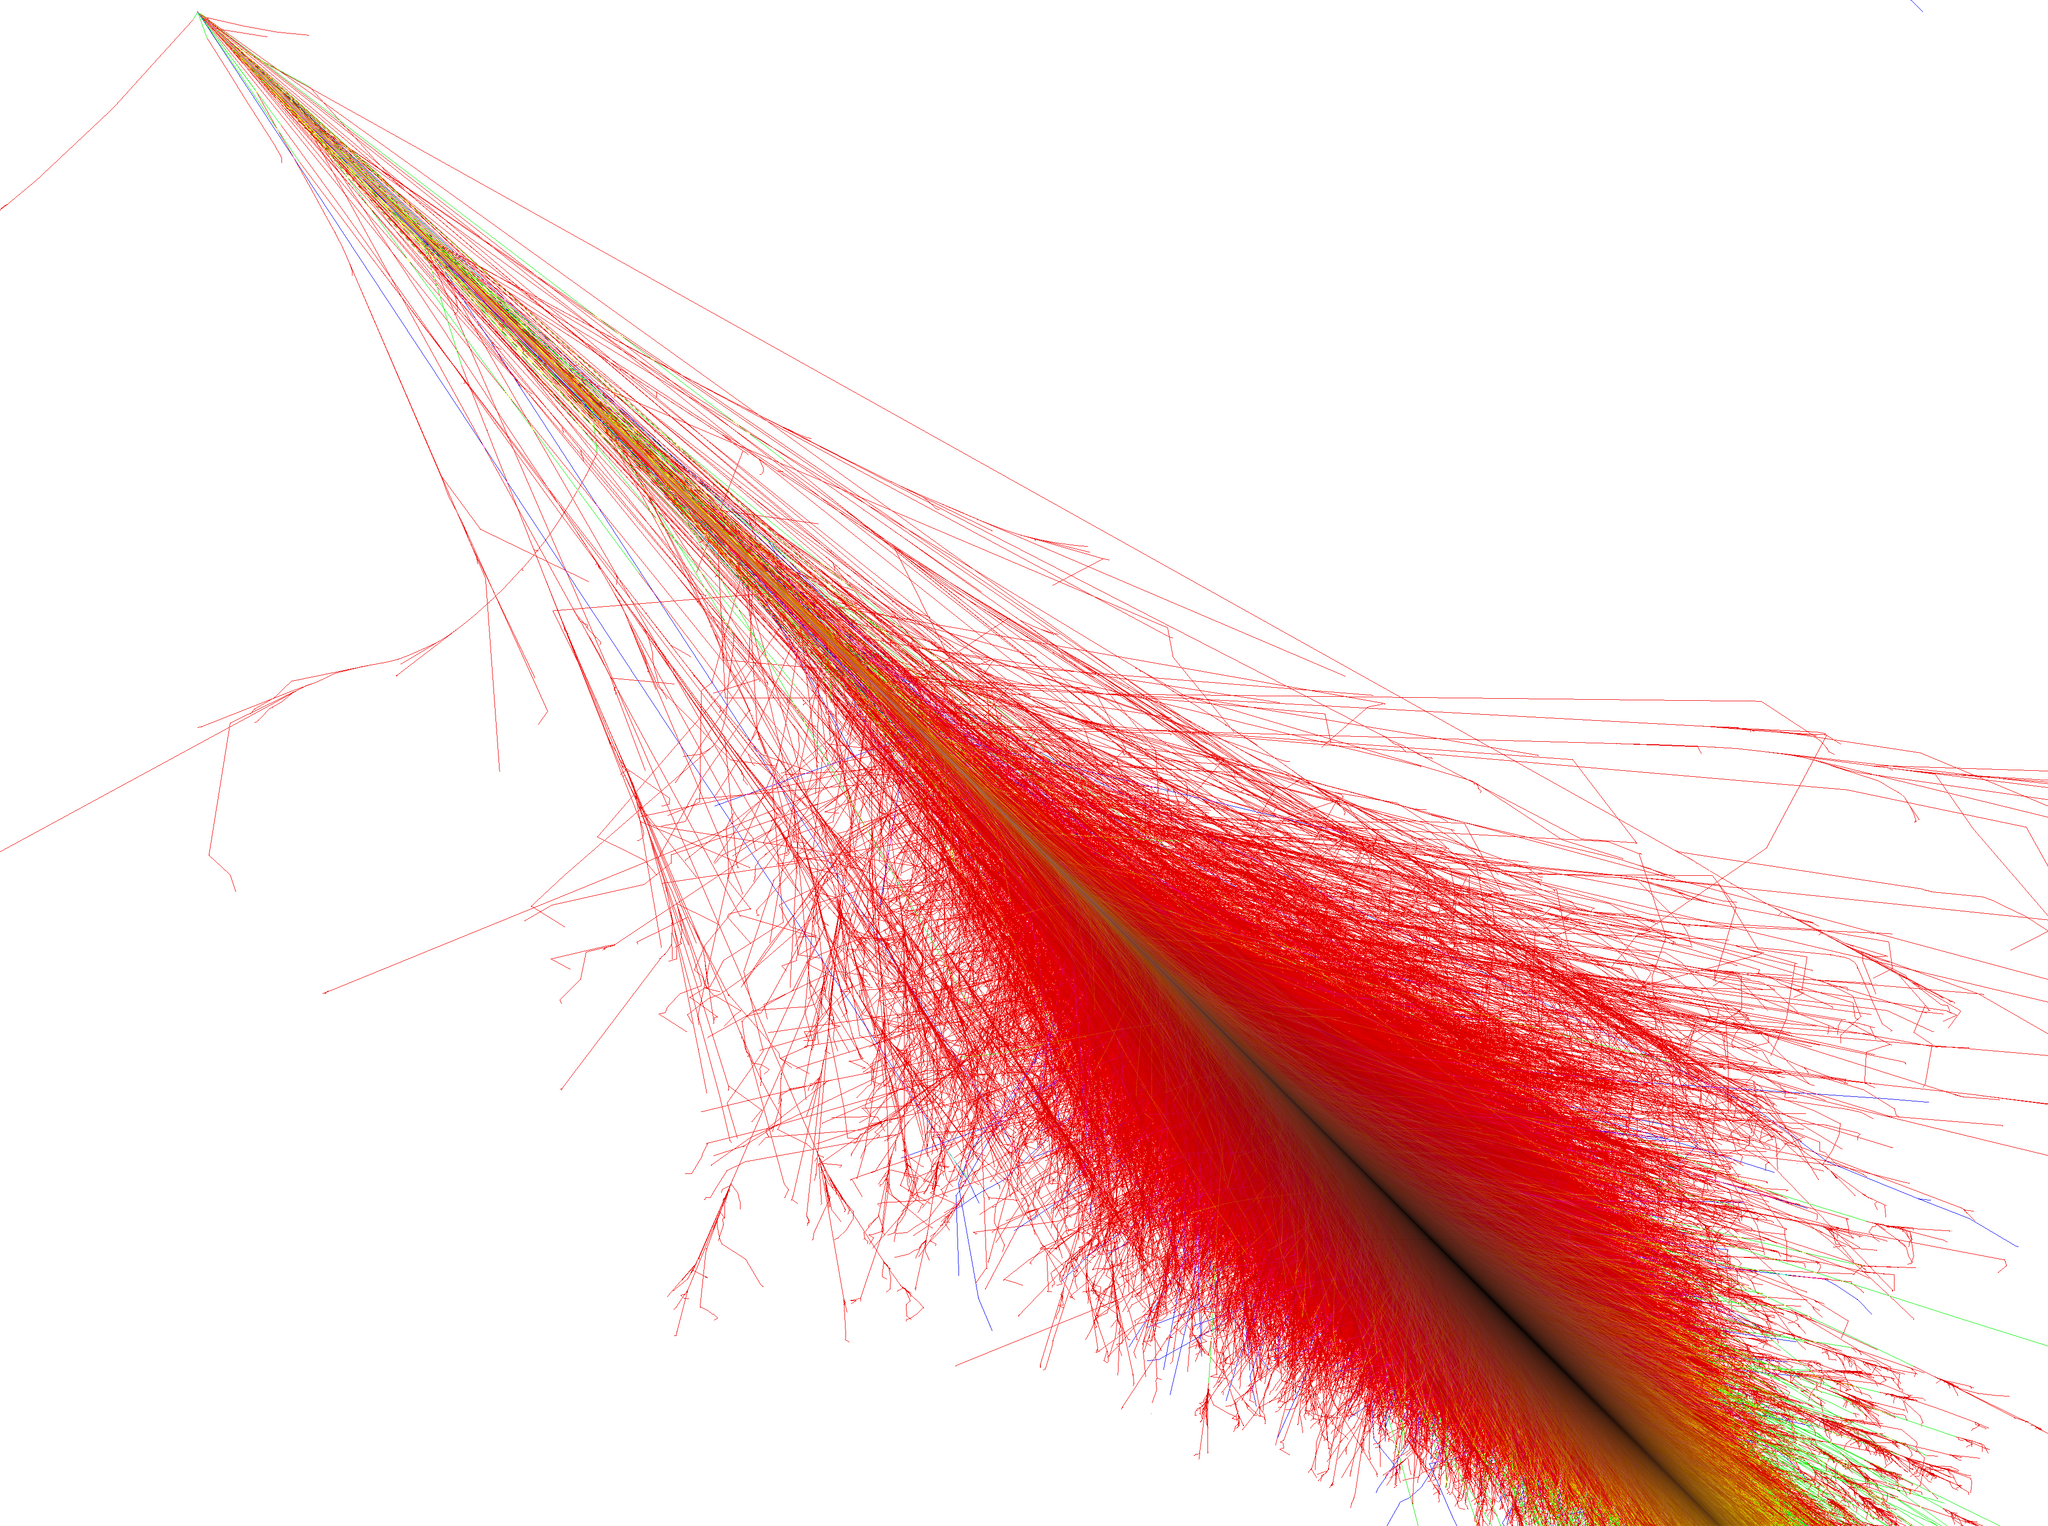
\includegraphics[width=0.8\linewidth]{data/shower-45}
	\caption{Proton Air Shower \cite{corsika-images}}
	\label{fig:proton-shower}
\end{figure}
\todo{Decay channels}
\subsection{Detection methods}
\todo{scintillators}
\acrshort{eas} can be detected through a number of methods. One such method is to observe the Cherenkov radiation produced by the primary particle. This radiation occurs since the local speed of light in the visible spectrum is lower than its vacuum speed. Due to the high energy of the primary particle its speed is nearly $1c_0$. This causes an effect comparable to a mach cone for supersonic objects in air and is known as Cherenkow radiation. This radiation is in the UV spectrum and can be observed at the surface of earth for example with an array of sensitive telescopes. One such array is HESS, located in Namibia. \\
Also detectable is the electromagnetic component of the showers, since its spectrum has a peak in the radio range and this penetrates deeply into the atmosphere. This can be picked up by a range of radio antenna. \\
Another method is to detect the muonic component. Muons ($\mu$) are elementary particles, often called the heavy sibling of the electron. It also has a charge of $-1$, a spin of $\frac{1}{2}$ but a much higher mass of
$105.6583755\,\si{MeV/c^2}$. It also only has a mean lifetime of $\snsi{2.1969811}{-6}{s}$. Muons only interact weakly with matter and thus penetrate deeply into the atmosphere. This fact has been used in the past to image large masses such as volcanoes and pyramids by a method called muon tomography.

\section{Detector Network}
The detector network is made up of a number of low-cost scintillator detectors. Each detector consists of a scintillator with \acrfull{sipm} assembly, an interface board with \acrfull{adc} and a RaspberryPi minicomputer. The interface board analyses signals from the \acrshort{sipm}, retrieves the current timestamp and passes this timestamped event along to a software running on the RaspberryPi minicomputer which sends it to a server. Each timestamped event is thus written to a central database where it can be further analysed at a later time. Due to the number of detectors and their respective rate of few Hz, a large number of events is writen to the database. This causes a large strain on the server infrastructure when running post-analysis programs since they need to handle large amounts of data in a short period of time. Since this is sub-optimal, a realtime solution which performs as much analysis and pre-filtering as possible in order to reduce the runtime impact of the analysis is preferable.

\section{Real-time analysis}
\subsection{Coincidence criteria}
A sturdy criterium to define a coincidence has to be found. Initially the criterium was defined as the $\Delta{t}$ of two events being lower than $100\,\mu\text{s}$, which corresponds to a maximum possible detector distance of $29.97\,\text{km}$. Since in reality the maximum coincidence interval is dependent on the actual detector distance and is limited by the flight distance of a muon, this criterium must be improved upon. A first approach thereby lies in calculating the distance between the detector pair belonging to the coincidence event which is to be analysed. This is implemented as the euclidean distance derived from the detector coordinates. Therefore the WGS84 earth coordinate model has been implemented to be able to convert a given pair of geodetic coordinates to relative carthesian coordinates, specifically in the \acrfull{enu} system. The WGS84 model thereby approximates the shape of earth as an oblate spheroid. Given the straight line distance, the time of flight given the speed of light in vacuum $c_0$ can be taken as a first approximation for the expected maximum coincidence window.

This value however still needs to be refined in two ways. firstly, a minimum value has to be set due to limitations of the possible time resolution of the timestamping of each event and a not well understood per-detector timing offset on the order of magnitude of few tens of ns. This is especially critical in the case of detectors which are close together, since their calculated time of flight is only few ns, and thus would cut off a significant number of coincidence events. In order to mitigate this, a minimum coincidence window of $150\,\text{ns}$ width is defined. This value is chosen to reliably capture all coincidence events for even the closest detector pairs.

A maximum upper coincidence window width has to be defined too, though this requires a more in depth analysis. Following influences have to be considered:
\begin{itemize}
	\item maximum expected zenith angle of muons
	\item maximum flight distance for a muon of maximum expected energy
	\item Muon flux cutoff value
\end{itemize}
\subsubsection*{Zenith angle}
The muon flux after the zenith angle can be described by \todo{function for distribution} distribution\cite{muonenergyspectrum} which can be approximated by a $\cos^2$ function. A cutoff of relative intensity of $1\,\%$ is chosen for the maximum zenith angle which leads to an angle of $\theta_{max} = \arccos\left(\sqrt{1\,\%}\right) = 84\,^\circ$.
\subsubsection*{Energy cutoff}
\subsubsection*{Muon Flux cutoff}
The muon flux cutoff value is chosen so that the frequency of the muons which are lost is below a threshold of $1\,\frac{1}{\text{a}}$. This frequency is determined through the muon spectrum\cite{muonenergyspectrum} at a zenith angle of $\theta = 0^{\circ}$. 
\subsection{Coincidence and plausability determination}
In order to determine coincidences, each event needs to be checked against all other events which are currently in the event buffer. To do this, the 
\section{Program layout}
The path of an event in the program is shown in figure \ref{fig:programlayout}. The source receives the event data and passes it on to the Station supervision class. It supervises the runtime data of each detector station and classifies it into reliability states. The specific criteria are described in the flowchart in figure \todo{make flowchart}.
\begin{figure}
	\centering
	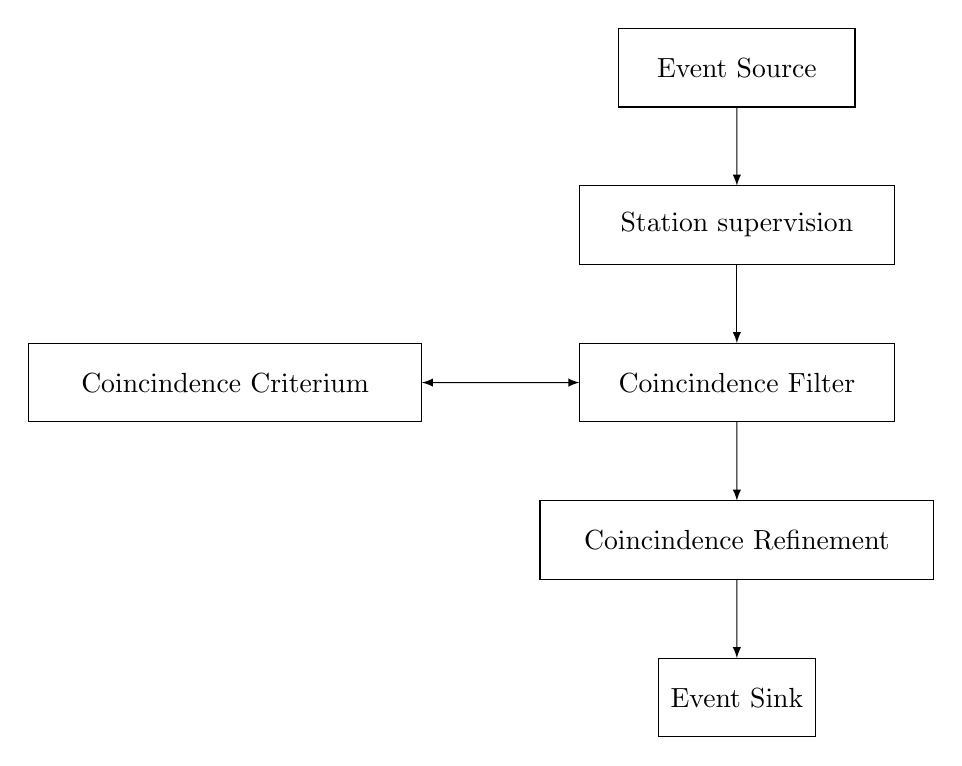
\begin{tikzpicture}
		\draw (-0.5,0) rectangle++(3,1) ++ (-1.5,-0.5) node {Event Source} ++ (0,-0.5) coordinate(esourceout);
		\draw (-1,-2) rectangle++(4,1) ++ (-2,-0.5) node {Station supervision} ++ (0,0.5) coordinate(stationsin) ++ (0,-1) coordinate(stationsout);
		\draw (-1,-4) rectangle++(4,1) ++ (-2,-0.5) node {Coincindence Filter} ++ (0,0.5) coordinate(coincfin) ++ (0,-1) coordinate(coincfout) ++ (-2,0.5) coordinate(coincfleft);
		\draw (-1.5,-6) rectangle++(5,1) ++ (-2.5,-0.5) node {Coincindence Refinement} ++ (0,0.5) coordinate(coincrin) ++ (0,-1) coordinate(coincrout);
		\draw (0,-8) rectangle++(2,1) ++ (-1,-0.5) node {Event Sink} ++ (0,0.5) coordinate(esinkin);
		
		\draw (-8,-4) rectangle++(5,1) ++ (-2.5,-0.5) node {Coincindence Criterium} ++ (2.5,0) coordinate(coinccin);
		
		\draw[->, >=latex] (esourceout) -- (stationsin);
		\draw[->, >=latex] (stationsout) -- (coincfin);
		\draw[->, >=latex] (coincfout) -- (coincrin);
		\draw[->, >=latex] (coincrout) -- (esinkin);
		\draw[<->, >=latex] (coincfleft) -- (coinccin);
	\end{tikzpicture}
	\caption{Program layout}
	\label{fig:programlayout}
\end{figure}
\backmatter
\end{document}
